\providecommand{\main}{../../../..}
\documentclass[\main/dresen_thesis.tex]{subfiles}

\begin{document}
  \label{sec:looselyPackedNS:nanoparticle:xrd}
  \begin{figure}[tb]
    \centering
    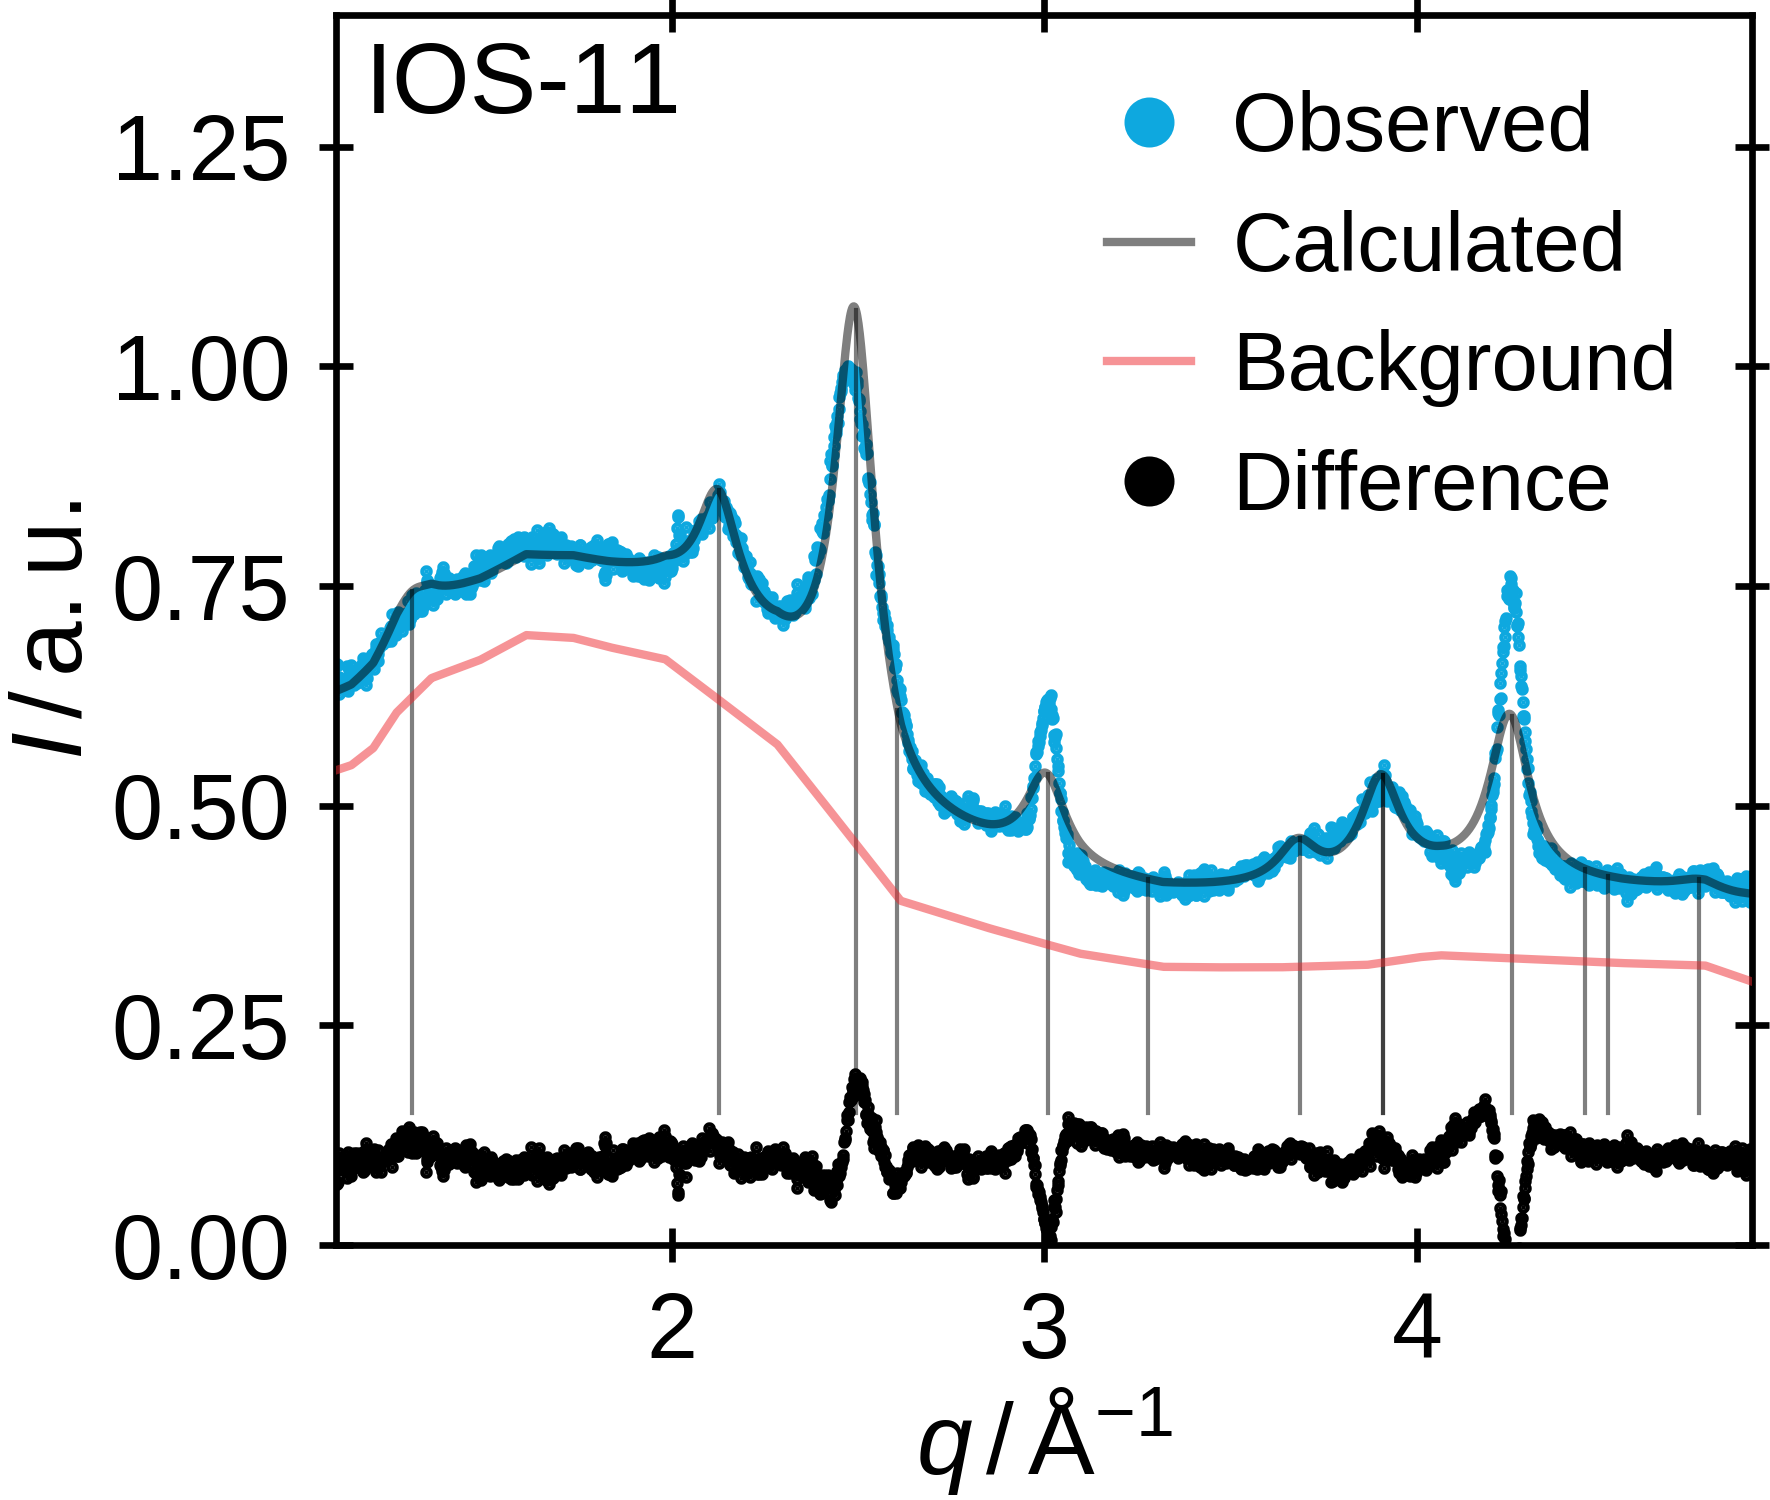
\includegraphics{looselyPackedNP_XRD_Fe2O3IOS-11}
    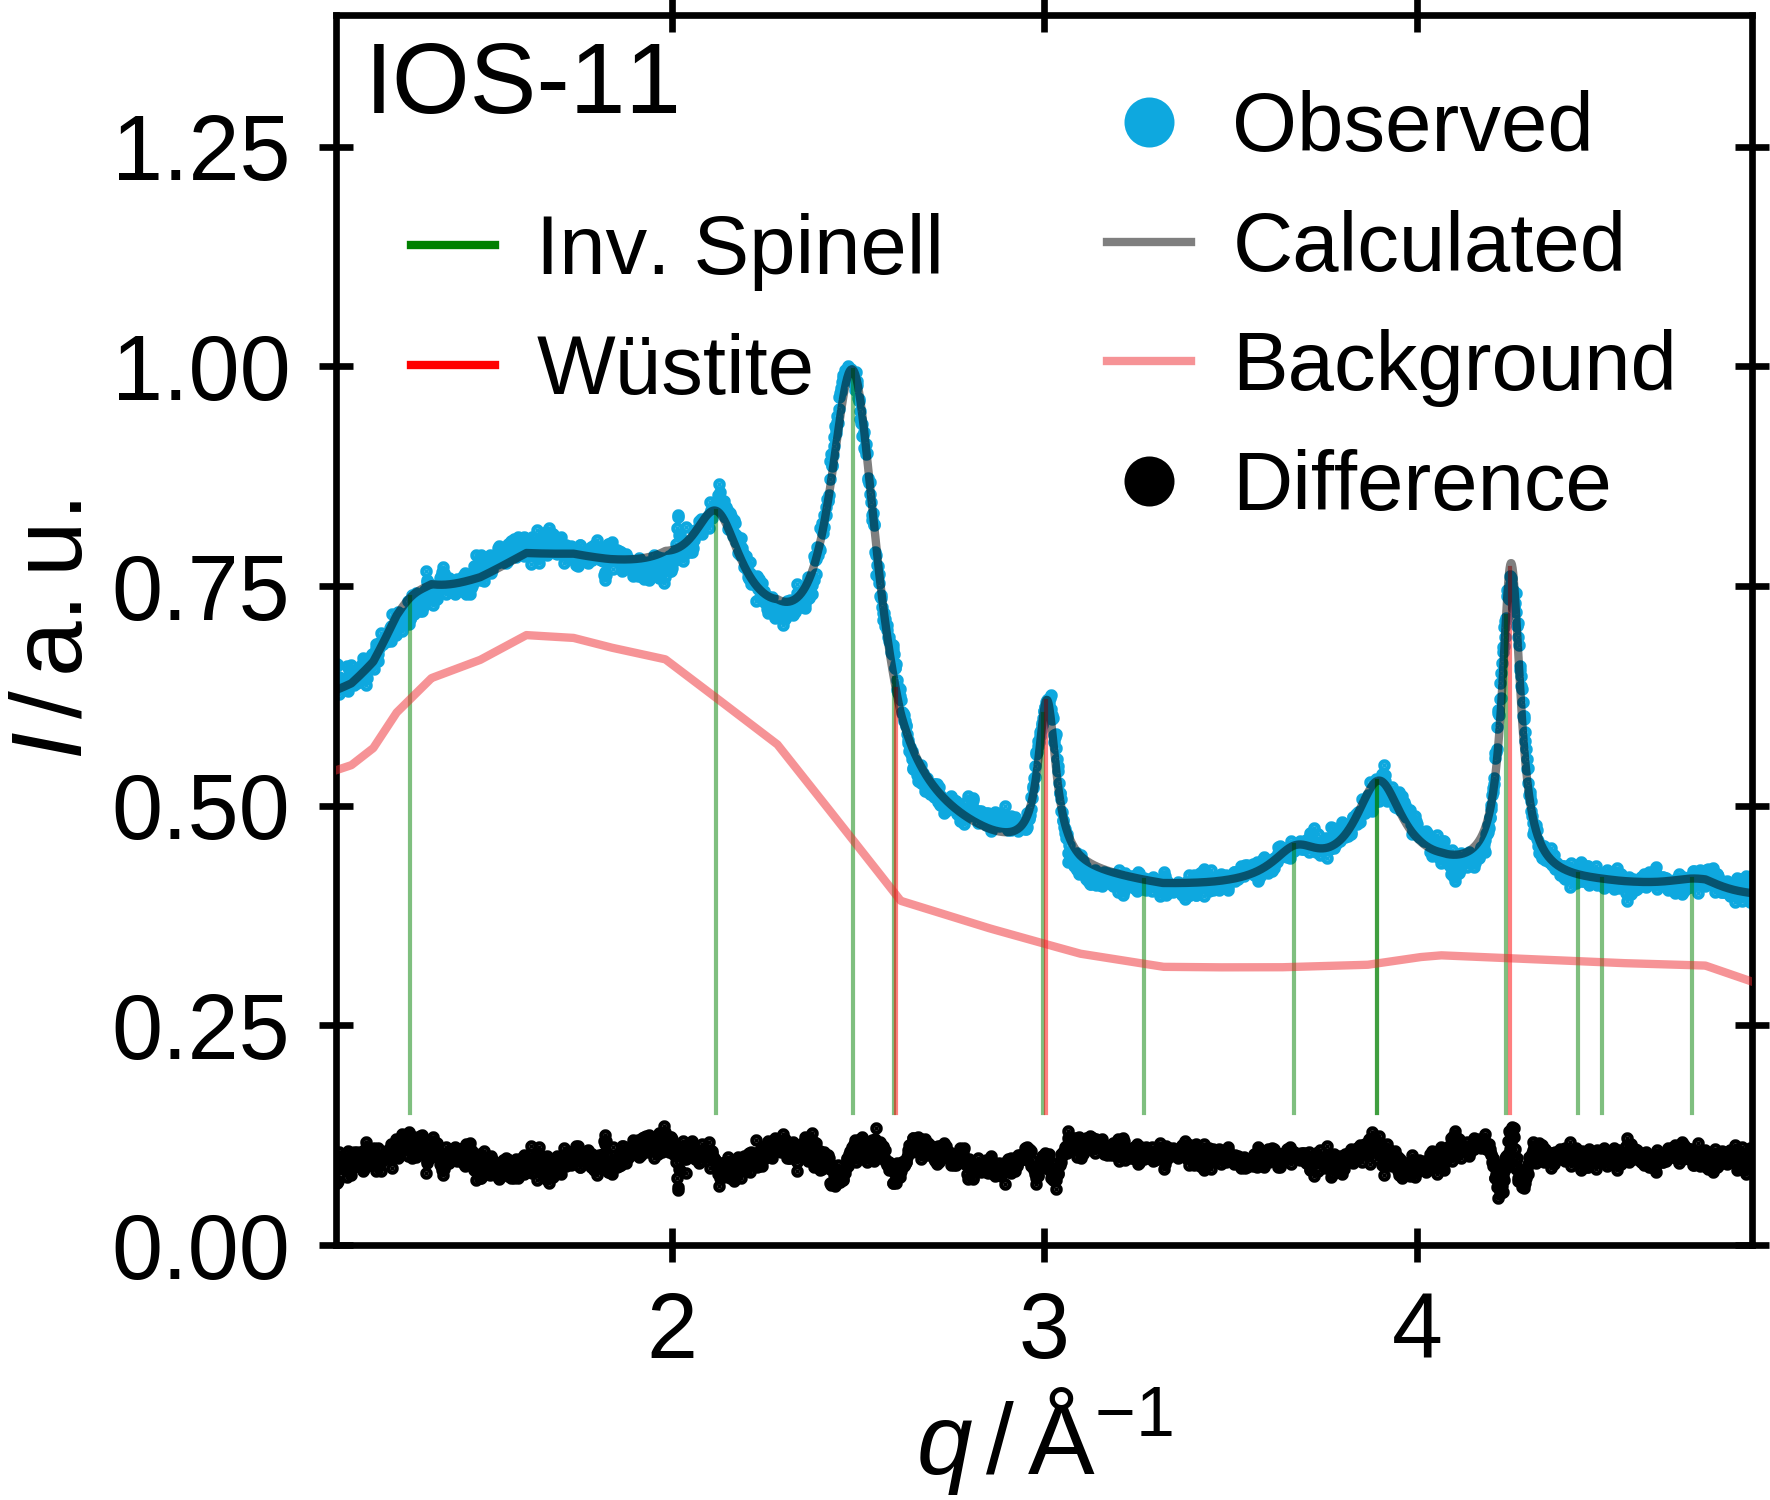
\includegraphics{looselyPackedNP_XRD_Fe2O3WustiteFit_IOS-11}
    \caption{\label{fig:looselyPackedNP:nanoparticle:xrd}XRD of IOS-11, once with a LeBail fit of a inverse spinell phase (left) and once with a LeBail fit where a sum of an inverse spinell and a w\"ustite phase is assumed. The manually estimated background is shown as red line.}
  \end{figure}

  In \reffig{fig:looselyPackedNP:nanoparticle:xrd} the diffraction data of IOS-11, and two performed LeBail fits are shown, to determine the phase, the lattice constant and the average crystallite size of the particles.
  On the left a LeBail fit is refined, where only an inverse spinell phase as expected from maghemite or magnetite.
  On the right LeBail fit, a combination of inverse spinell and w\"ustite phases is refined.
  For both approaches the parameters of the refinement, the lattice constants $a$ and the Lorentzian isotropic size parameter $Y$ are summarized in \reftab{tab:looselyPackedNS:nanoparticle:discussion:xrdLeBail}.

  It is clearly visible in the LeBail fit of only a single phase that the LeBail fit does not properly describe the measured XRD data.
  The reflections around $3 \unit{\angstrom}$ and $4.2 \unit{\angstrom}$ are poorly described, as the data shows a sharper peak width in these cases.
  By adding the w\"ustite phase, these problems are alleviated and the whole range is well described.

  \begin{table}[ht]
    \centering
    \caption{\label{tab:looselyPackedNS:nanoparticle:discussion:xrdLeBail}LeBail refinement parameters for the two fits to IOS-11 shown in \reffig{fig:monolayers:nanoparticle:xrd}. Given are the parameters of the lattice constants $a$ and the Lorentzian isotropic size parameter $Y$ for each phase. Additionally, the calculated crystallite size $L$ from the Debye-Scherrer equation is given for each phase, as well as the wavelength $\lambda$ used at each measurement, the figure of merit $\chi^2$ and the agreement factors $R$.}
    \begin{tabular}{ l | l | l }
      \hline
      \rule{0pt}{2ex} & \multicolumn{2}{c}{\textbf{IOS-11}}\\
      \hline
      \hline
      \rule{0pt}{2ex}space group & $Fd\bar{3}m$ (No. 227) & + $Fm\bar{3}m$ (No. 225)\\
      \hline
      \rule{0pt}{2ex} $a_\mathrm{inv. spinell} \,/ \unit{\angstrom}$         & $8.3729(4)$ & $8.3843(3)$  \\
      \rule{0pt}{2ex} $Y_\mathrm{inv. spinell} \,/ \unit{^\circ}$            & $1.778(8)$  & $2.198(5)$   \\
      \rule{0pt}{2ex} $a_\textsf{w\"ustite}     \,/ \unit{\angstrom}$        &             & $4.1819(1)$  \\
      \rule{0pt}{2ex} $Y_\textsf{w\"ustite}     \,/ \unit{^\circ}$           &             & $0.755(3)$   \\
      \hline
      \rule{0pt}{2ex} $L_\mathrm{inv. spinell} \,/ \unit{nm}$                & $3.161(1)$  & $2.557(1)$ \\
      \rule{0pt}{2ex} $L_\textsf{w\"ustite}      \,/ \unit{nm}$              &             & $7.442(2)$ \\
      \hline
      \rule{0pt}{2ex} $\lambda \,/ \unit{\angstrom}$                         & \multicolumn{2}{c}{$1.54056$}\\
      \hline
      \rule{0pt}{2ex} $\chi^2$                                               & $7.00$      & $1.70$ \\
      \rule{0pt}{2ex} $R_p \,/ \unit{\%}$                                    & $2.52$      & $1.52$ \\
      \rule{0pt}{2ex} $R_{wp} \,/ \unit{\%}$                                 & $3.93$      & $1.94$ \\
      \rule{0pt}{2ex} $R_{exp} \,/ \unit{\%}$                                & $1.49$      & $1.48$ \\
      \rule{0pt}{2ex} $R_{f, \, \mathrm{inv. spinell}} \,/ \unit{\%}$        & $0.15$      & $0.10$ \\
      \rule{0pt}{2ex} $R_{f, \, \text{w\"ustite}} \,/ \unit{\%}$             &             & $0.15$ \\
      \hline
    \end{tabular}
  \end{table}

    The nanoparticle IOS-11 shows two phases, an inverse spinell phase with a lattice constant of $8.3843(3) \unit{\angstrom}$ and a w\"ustite phase with a lattice constant of $4.1819(1) \unit{\angstrom}$.
    These values can be compared to the bulk values of the lattice constant of magnetite/maghemite ($a_\mathrm{magnetite} \eq 8.396 \unit{\angstrom}$, $a_\mathrm{maghemite} \eq 8.340 \unit{\angstrom}$) \cite{Cornell_2003_Their} and to the bulk value of w\"ustite ($a_\mathrm{FeO} \eq 4.33 \unit{\angstrom}$ \cite{Hentschel_1970_Stoich}).

    The observed lattice constant for the inverse spinell phase lies in between the bulk values of magnetite and maghemite, and the lattice constant of the w\"ustite phase is significantly below that of the bulk literature value.
    This can be compared to the study of the oxidation of iron oleate nanoparticles by Wetterskog \etal \cite{Wetterskog_2013_Anoma}.
    For the as-synthesized nanocubes a lattice constant of $4.265 \unit{\angstrom}$ is found for the w\"ustite phase, which decreases in size upon oxidation.
    After full oxidation, a significant difference in the reflection width at $3 \unit{\angstrom}$ and $4.2 \unit{\angstrom}$ in comparison to the remaining reflections is still observed and attributed to a discrepancy between the long-range order of the tetrahedral and octahedral sublattice due to a topotaxial oxidation and formation of anti-phase boundaries in the volume of the nanoparticles \cite{Wetterskog_2013_Anoma}.
    The small w\"ustite lattice constant observed therefore indicates that the refined inverse spinell/w\"ustite structure in XRD is a phenomenological description for an actually fully oxidized nanoparticle in an inverse spinell phase with anti-phase boundaries in the volume.

    From the lattice constant of the inverse spinell phase, the assumption can be made that the shell is close to a magnetite phase as the value is closer to bulk magnetite in comparison to bulk maghemite \cite{Cervellino_2014_Latti}.
    For the continuing discussion of the nanoparticle structure and magnetism it is therefore assumed that $\delta \eq 0$ in the formula unit \ch{Fe_{3 - $\delta$}O4} .
    The mass density of the nanoparticle is in this case for the given inverse spinell lattice constant $\rho \eq 5.22 \unit{g\, mL^{-1}}$.
    As the precision of determining the oxidation state from the lattice parameter is however small, especially for small sized crystallite sizes, it has to be kept in mind that this assumption introduces a potential systematic error.
    \\

    From the Lorentzian isotropic size parameters, the crystallite sizes are determined to $7.442(2) \unit{nm}$ for the w\"ustite phase and $2.557(1) \unit{nm}$ for the inverse spinell phase.
    The obtained sizes from XRD are comparable to the total particle size observed in TEM ($10.95(5) \unit{nm}$).
    The sum of the core and two times the shell thickness, which amounts to $12.556(2) \unit{nm}$ is larger than the size from TEM, which due to the spherical shape of the nanoparticles is another indication that the two phases do not represent a core-shell structure but actually the discrepancy between the tetrahedral and octahedral sublattices.

  % \paragraphNewLine{Density}
  %   Due to the partial oxidation of the shell and the complex core-shell structure, the density can only be roughly estimated.

  %   To avoid introducing systematic errors by assuming a wrong phase of the shell, the density can be given by 5.2(1) g/mL
\end{document}